%!TEX root = ./abstracts/abstract.tex
\chapter{Programme}


\phantomsection\section*{Conférences plénières}

%%%%%%%%%%%%%%%%%%% Mardi 1er juin 10h -> 11h

\phantomsection\subsection*{Contraintes de manipulation des « nouveaux » combustibles dans les auxiliaires de turbines à gaz}
%
\begin{center}
Mardi 1er juin 2021 -- 10h
\end{center}

\hspace{0.04\linewidth}\vrule\hspace{0.01\linewidth}\parbox{0.88\linewidth}{
\textbf{{\scshape Pierre Montagne}\\ General Electric, Division Gas Power, Belfort}\\
{\slshape  Originaire de Nancy, Pierre Montagne devient Ingénieur en mécanique diplômé de Supméca Paris en 2008. Après un projet de fin d’étude dans les moteurs d’avions au sein de Rolls-Royce, a intégré GE en 2008 dans les auxiliaires turbines à gaz de la division Gas Power. Il est spécialisé dans les systèmes auxiliaires de conditionnement et d’injection de combustibles alternatifs dans le cadre de projets complexes (gaz de synthèse, hydrogène, traitement de combustibles liquides contaminés). Il enseigne aussi la combustion au sein du Master Ingénierie Thermique et Energie à Belfort depuis 2018-2019.}}\\[2ex]

\vspace{1cm}

La turbine à gaz est un convertisseur d’énergie réputé pour être capable de fonctionner avec un panel de combustibles très vaste, aussi bien liquides que gazeux. Dans le cadre des engagements de la lutte contre le changement climatique, les ambitions de décarbonation de l’industrie et de la production électrique vont ouvrir des perspectives d’utilisation d’une part croissante de « nouveaux » combustibles, d’hydrogène, d’ammoniac, de biogaz et de biocarburants. Ces « nouveaux » combustibles ne sont pas nouveaux par leur formulation, mais plutôt par l’ampleur de leur possible démocratisation et de l’opportunité qu’ils représentent, notamment pour alimenter des centrales thermiques. Ils ont des compositions chimiques différentes des carburants traditionnels et leur utilisation pure ou bien diluée dans ces derniers vont faire apparaître des propriétés physiques et des risques propres qu’il s’agit d’étudier en vue de préparer les adaptations nécessaires des systèmes auxiliaires de ces centrales. En particulier, les risques d’explosion dans toutes les phases d’opération de la centrale et dans des conditions de process contraignantes ont besoin d’être anticipés à travers l’estimation de leur occurrence, de leur sévérité et des moyens de prévention et de contrôle à disposition.

\vspace{\stretch{1}}

%%%%%%%%%%%%%%%%%%%% Mardi 01/06 14h -> 15h
%
\clearpage
\phantomsection\subsection*{Conception des turbofans:  progrès et enjeux}
%
\begin{center}
Mardi 1er juin 2021 -- 14h
\end{center}

\hspace{0.04\linewidth}\vrule\hspace{0.01\linewidth}\parbox{0.88\linewidth}{
\textbf{{\scshape Charles Foulquié}\\Safran Aircraft Engines, Villaroche}\\
{\slshape Ingénieur chez Safran Aircraft Engines et enseignant vacataire à l'Ecole Nationale Supérieure d'Arts et Métiers, Charles Foulquié évolue dans le domaine des machines de conversion d'énergie depuis maintenant dix ans. Son domaine d’expertise consiste dans l'étude numérique des phénomènes acoustiques et vibratoires d’origine aérodynamique appliqué aux turboréacteurs.}}\\[2ex]

\vspace{1cm}

L’impact environnemental de l’aéronautique civile est une préoccupation croissante de nos sociétés. Afin de répondre à ces enjeux, les ingénieurs motoristes repoussent sans cesse les limites technologiques de leurs produits. Notamment, l’architecture moteur {\slshape turbofan} qui équipe de nos jours la flotte mondiale d’avion de ligne moyen et long-courriers est un concentré de technologie et d'innovation prodigieux. L’objet de cette conférence est d’introduire aux problématiques techniques et scientifiques rencontrés lors de la conception de ces moteurs. Une attention particulière est porté aux progrès réalisés sur le plan de l’efficacité énergétique et des nuisances acoustiques [1,2].

Le {\slshape turbofan} est une machine thermique basée sur le cycle thermodynamique de Joule-Brayton dont l’objectif est de produire une poussée par accélération d’un débit d’air. Son efficacité énergétique globale est conditionnée par son rendement thermodynamique d’une part ainsi que son rendement propulsif d’autre part. Le {\slshape fan} (voir figure) qui est responsable de 75\% de la poussée est l’un des éléments constitutifs du moteur les plus critiques vis-à-vis de l’efficacité énergétique globale. Il est également une source de nuisance acoustique de premier plan à l’échelle de l’aéronef. Sa conception fait l’objet de recherches actives à la frontière entre aérodynamique, acoustique et mécanique vibratoire [3]. Une partie substantielle de la conférence lui est dédiée.

\begin{center}
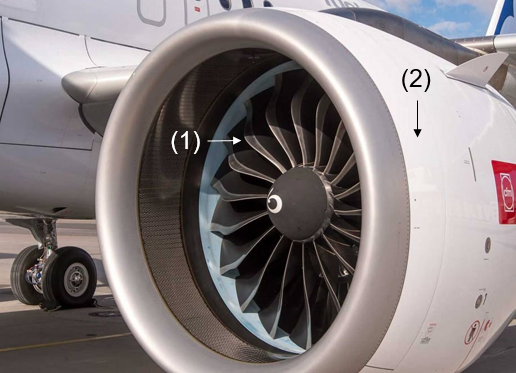
\includegraphics[height=5cm]{../Logos/Turbofan.png} \\
Figure 1 : Fan$^1$ et entrée d’air$^2$ du turbofan Leap-1A équipant l’Airbus A320Neo. 
\end{center}

\noindent [1] La saga du CFM 56, Arts et Métiers Alumni, 23 octobre 2017, Pierre Alesi et Patrick Joyez.\\
\noindent [2] Advanced Air Transport Technology Project, Acoustic Considerations for PAI, NASA.\\
\noindent [3] Aero-engine design: a state of the art Fan Aerodynamic Design, VKI lecture series, April 7-11, 2003, Jérôme Lépine.

%
%

%%%%%%%%%%%%%%%%%%% Mercredi 2 juin 09h -> 10h
\clearpage
\phantomsection\subsection*{Systèmes de propulsion intégrés énergétiquement pour les automobiles}
%
\begin{center}
Mercredi 2 juin 2021 -- 09h
\end{center}

\hspace{0.04\linewidth}\vrule\hspace{0.01\linewidth}\parbox{0.88\linewidth}{
\textbf{{\scshape Zlatina Dimitrova}\\ Cheffe de Projet en Recherche et Innovation, Direction Recherche Innovation \& Ingénierie avancée, Stellantis, Vélizy}\\
{\slshape Dr. Zlatina Dimitrova travaille dans l’industrie automobiles, chez Stellantis (ex-PSA Groupe) en tant que Cheffe de Projet en Recherche et Innovation, dans le domaine de l’énergie et de la propulsion automobile. Zlatina a obtenu son Habilitation à Diriger des Recherches en 2020 au CNAM Paris. Elle détient également un doctorat de l’Ecole Polytechnique Fédérale de Lausanne (Suisse).}}\\[2ex]

\vspace{1cm}
Le fil conducteur dans cette présentation est l'amélioration de l'efficacité des systèmes énergétiques des véhicules, la réduction de leurs émissions, au travers de solutions compétitives et rentables de technologies de stockage et de conversion d'énergie. La recherche porte sur l'efficacité énergétique ainsi que sur les études d'impacts économiques et environnementaux des systèmes énergétiques innovants. Dans cette présentation les systèmes énergétiques des véhicules évoluent des systèmes autonomes embarqués vers des systèmes liés au réseau, avec des vecteurs multi-énergies. Trois grands thèmes de recherche sont développés : 
\begin{itemize}[label=\textbullet]
    \item Efficacité énergétique, stockage et conversion à bord des véhicules
    \item Extension des systèmes énergétiques des véhicules, les véhicules en tant que systèmes liés au réseau
    \item Systèmes de stockage et de conversion d'énergie pour les différents vecteurs énergétiques; véhicules électriques à pile à combustible, hydrogène et leur écosystème
\end{itemize}
Pour prendre en compte l'impact des différents vecteurs énergétiques, le bilan du puits à la roue de l'efficacité énergétique et des émissions de $\unit{CO_2}$ est réalisé et discuté pour différents systèmes de propulsion des véhicules. L’impact du mix énergétique est ainsi recensé sur les émissions de $\unit{CO_2}$ des différents systèmes énergétiques des véhicules. La production de l’hydrogène propre ou encore vert est également abordée, en lien avec le mix énergétique. 


%%%%%%%%%%%%%%%%%%% Jeudi 3 juin 9h30 -> 10h30
\clearpage
\phantomsection\subsection*{Panorama des activités EDF R\&D face aux enjeux énergétiques}
%
\begin{center}
Jeudi 3 juin 2021 -- 9h30
\end{center}

\hspace{0.04\linewidth}\vrule\hspace{0.01\linewidth}\parbox{0.88\linewidth}{
\textbf{{\scshape Franck David}\\ EDF - EDF R\&D, Mécanique des Fluides, Energies, Environnement, Chatou}\\
{\slshape Franck DAVID est Chercheur Senior à EDF R\&D dans le domaine des échangeurs thermiques et des cycles de conversion d’énergie pour la production. Il intègre EDF en 1991 pour travailler au développement, la qualification et ainsi qu’à la réalisation des premières études du Code THYC Echangeurs (échelle 3D diphasique poreux) appliqué aux Générateurs de Vapeur et aux Condenseurs. Il a exercé des activités de management d’équipes en charge de modélisation et d’expérimentation et de pilotage de projet au sein de la R\&D. Depuis 2010, il travaille en tant qu’expert dans le domaine des Nouveaux Réacteurs, des Systèmes de refroidissement pour la production et pour la Sûreté. Il a participé à différents programmes Européens dans le domaine des réacteurs Sodium, des technologies de refroidissement et des Technologies de Sûreté Passive. Il a encadré 3 thèses, produit une vingtaine de communications, est membre de la SFEN, de la SFT  et du Conseil d’administration de l’association GRETH. Il intervient ponctuellement dans des activités d’enseignement.}}\\[2ex]

\vspace{1cm}

L'entreprise EDF est un acteur majeur du monde de l'énergie en France et dans le monde. Ses activités sont multiples et couvrent les métiers de la production, du transport et de la distribution d'électricité ainsi que la commercialisation d'énergie et de service énergétique. La R\&D d’EDF est une R\&D « intégrée » organisée pour répondre aux différents enjeux de l'entreprise exprimés dans le cadre du plan stratégique de l'entreprise CAP 2030 et pour préparer les systèmes de productions du futur dans le cadre de la PPE et de la nécessaire réduction des émissions de gaz à effets de serre.

L'objet de la présentation est de fournir un éclairage sur les principales activités de la R\&D pour répondre à ces enjeux en présentant succinctement les grandes orientations de son plan scientifique et en illustrant son programme d'activité par quelques exemples de réalisation ou des travaux de recherche en cours dans les domaines de l'énergétique et de la thermique appliqués à la production décarbonée ou aux usages.


%%%%%%%%%%%%%%%%%%% Jeudi 3 juin 16h - 17h
\clearpage
\phantomsection\subsection*{La loi constructale et le stockage thermique}
%
\begin{center}
Jeudi 3 juin 2021 -- 17h
\end{center}

\hspace{0.04\linewidth}\vrule\hspace{0.01\linewidth}\parbox{0.88\linewidth}{
\textbf{{\scshape Sylvie Lorente }\\ Department of Mechanical Engineering, Villanova University, Pennsylvania, USA}
\\
{\slshape Sylvie Lorente est le Chair Professor du Collège d’Ingénierie dans le département de Mécanique à Villanova University, PA, USA et Professeur à l’INSA Toulouse, département Génie Civil. Elle est member de l’Académie Européenne. Sylvie est passionée par les architectures d’écoulement et travaille sur les structures vascularisées, les milieux poreux, le design et les organisations urbaines. Elle est l’auteur de 7 livres, 10 chapitres d’ouvrages et 200+ articles dans des revues internationales. Elle est éditeur de International Communications in Heat and Mass Transfer et membre de plusieurs comités éditoriaux. Elle figure parmi les 2\% des scientifiques les plus cités au monde. }
}\\[2ex]

\vspace{1cm}

Enoncée en 1996 par Adrian Bejan, la loi constructale a depuis vu son potentiel d’application s’élargir dans les diffèrent domaines de l’ingénierie, mais aussi vers d’autres horizons scientifiques tels que la physique, la biologie, la médicine, les sciences sociales, l’économie, etc. L’idée que les architectures d’écoulement s’adaptent dans le temps pour survivre en modifiant leur configuration, si elle est née en thermodynamique, est suffisamment puissante pour s’étendre vers l’explication de nombreux autres phénomènes, qu’ils soient naturels ou issus de notre imagination. De fait, la loi constructale a aussi donné très rapidement lieu à des approches originales de design.

Dans cette présentation, j’aurai le plaisir d’illustrer quelques applications que nous avons développées dans le domaine du stockage de l’énergie et des matériaux à changements de phase. Augmenter la part de la contribution des énergies renouvelables dans le mix énergétique nécessite d’accomplir des progrès dans diverses directions: remporter l’adhésion des citoyens, des mesures politiques, technologiques et des avancées scientifiques pour n’en mentionner que quelques-uns. L’un des plus grands défis consiste à offrir des solutions intelligentes pour résoudre la dichotomie entre la production d’énergie et les périodes de consommation sachant que l’écart couvre plusieurs échelles de temps. C’est tout l’objet du stockage thermique.

L’approche constructale du design de systèmes à changement de phase sera d’abord présentée. Nous montrerons que lorsque le temps de stockage est fixé, de même que le volume de matériau à changement de phase, le fluide caloporteur peut être distribué dans le volume de manière à utiliser les mécanismes de transfert de chaleur quand et où ils sont le plus efficaces. Les réacteurs de stockage thermochimiques sont un autre domaine dans lequel la loi constructale trouve tout son sens pour le design de réacteurs plus compacts et efficaces. Nous verrons que l’emplacement des sels peut être choisi pour décroître les imperfections thermodynamiques. 


%%%%%%%%%%%%%%%%%%%%%%%%%%%%%%%%%%%%%%%%%%%%%%%%%%%%%%
\newpage
\phantomsection\section*{Ateliers}
%%%%%%%%%%%%%%%%%%%%%%%%%%%%%%%%%%%%%%%%%%%%%%%%%%%%%%


%%%%%%%%%%%%%%%%%%% Mardi 2 juin 15h30 -> 16h30
%\clearpage
\phantomsection\subsection*{Climat}
%
\begin{center}
Mardi 2 juin 2021 -- 15h30
\end{center}

\hspace{0.04\linewidth}\vrule\hspace{0.01\linewidth}\parbox{0.9\linewidth}{
\textbf{{\scshape Frédéric André} -- INSA de Lyon, CETHIL, Lyon}\\
\textbf{{\scshape Cyril Caliot} -- Université de Pau et des Pays de l’Adour, LMAP - Laboratoire de Mathématiques et de leurs Applications, Pau}\\
\textbf{{\scshape Nicolas Ferlay} -- Université de Lille, LOA - Laboratoire d’Optique Atmosphérique, Villeneuve d'Ascq}
%\textbf{{\scshape Laurent Ibos} -- CERTES, Créteil}\\
%\textbf{{\scshape Jean-Luc Bailleul} -- LTeN, Nantes}\\
%\textbf{{\scshape Jean Dumoulin} -- IFFSTAR, Nantes}\\
%\textbf{{\scshape Bertrand Garnier} -- LTeN, Nantes}
}\\[2ex]

\vspace{1cm}
\hrule
%%%%%%%%%%%%%%%%%%% Mardi 2 juin 15h30 -> 16h30
%\clearpage
\phantomsection\subsection*{Concours CNU 62 – CNRS section 10}
%
\begin{center}
Mardi 2 juin 2021 -- 15h30
\end{center}


\hspace{0.04\linewidth}\vrule\hspace{0.01\linewidth}\parbox{0.9\linewidth}{
\textbf{{\scshape Souad Harmand} -- Université Polytechnique des Hauts de France, LAMIH, Valenciennes}\\
\textbf{{\scshape Jean-Luc Battaglia} -- Université de Bordeaux, I2M ENSAM, Talence}
}\\[2ex]


\vspace{1cm}
\hrule

%%%%%%%%%%%%%%%%%%% Jeudi 3 juin 1100 -> 12h00
%\clearpage
\phantomsection\subsection*{Hydrogène-énergie}
%
\begin{center}
Mercredi 3 juin 2021 -- 11h00
\end{center}


\hspace{0.04\linewidth}\vrule\hspace{0.01\linewidth}\parbox{0.9\linewidth}{
\textbf{{\scshape Nadia Steiner} -- Université de Franche-Comté, Femto-st, Fclab, Belfort}\\
\textbf{{\scshape Daniel Hissel} -- Université de Franche-Comté, Femto-st, Fclab, Belfort}\\
\textbf{{\scshape Olivier Joubert} -- Université de Nantes, Institut des matériaux Jean Rouxel, fédération FRH2, Nantes}}\\[2ex]

\vspace{1cm}
\hrule

%%%%%%%%%%%%%%%%%%% Jeudi 3 juin 1100 -> 12h00
%\clearpage
\phantomsection\subsection*{Propriétés thermophysiques -- Base de données}
%
\begin{center}
Mercredi 3 juin 2021 -- 11h00
\end{center}


\hspace{0.04\linewidth}\vrule\hspace{0.01\linewidth}\parbox{0.9\linewidth}{
\textbf{{\scshape Bernard Desmet} -- Université Polytechnique des Hauts de France, Valenciennes}}\\[2ex]

\vspace{1cm}
\hrule


%\subsubsection*{Conclusion}
%
%\hspace{0.04\linewidth}\vrule\hspace{0.01\linewidth}\parbox{0.9\linewidth}{
%\textbf{{\scshape Christophe Le Niliot} -- Aix-Marseille Université}
%}\\[2ex]
